\documentclass{article}

\usepackage[english]{babel}
\usepackage[utf8]{inputenc}
\usepackage{graphicx, float}
\usepackage{hyperref}
\usepackage[outdir=./]{epstopdf}
\usepackage{subcaption}


\title{Thesis}
\author{Filip Kronström}
\date{\today}

\begin{document}
\maketitle
\section{Method}
\subsection{Pose estimation - 2D}
The pose estimation is built around the open source framework MMPose \cite{mmpose} and it uses the \emph{Distribution-Aware coordinate Representation of Keypoint}, \textbf{DARK}, method \cite{Zhang2020} to extract the body joints from the images. The model used is trained on the \textbf{COCO} dataset \cite{Lin2014}. In this data set the human body is represented by 17 joints which can be seen in Figure \ref{fig:COCO-joints}. In Figure \ref{fig:joints-comparison} the estimated joints are shown together with joints measured by ... The difference in shoulder location in Figure \ref{fig:joints-comparison} can be explained by the positions of the joints tracked, which is also illustrated in Figure \ref{fig:COCO-joints}. This is something that is also reflected in the difference between the measured and estimated knee positions, shown in Figure \ref{fig:errors-2d}.

\subsection{Pose estimation - 3D}
- \cite{Pavllo2019}. Results not good atm, model needs finetuning with our depth data if used, see Figures \ref{fig:joints-comp3d}, \ref{fig:errors-3d}.

\begin{figure}
  \centering
  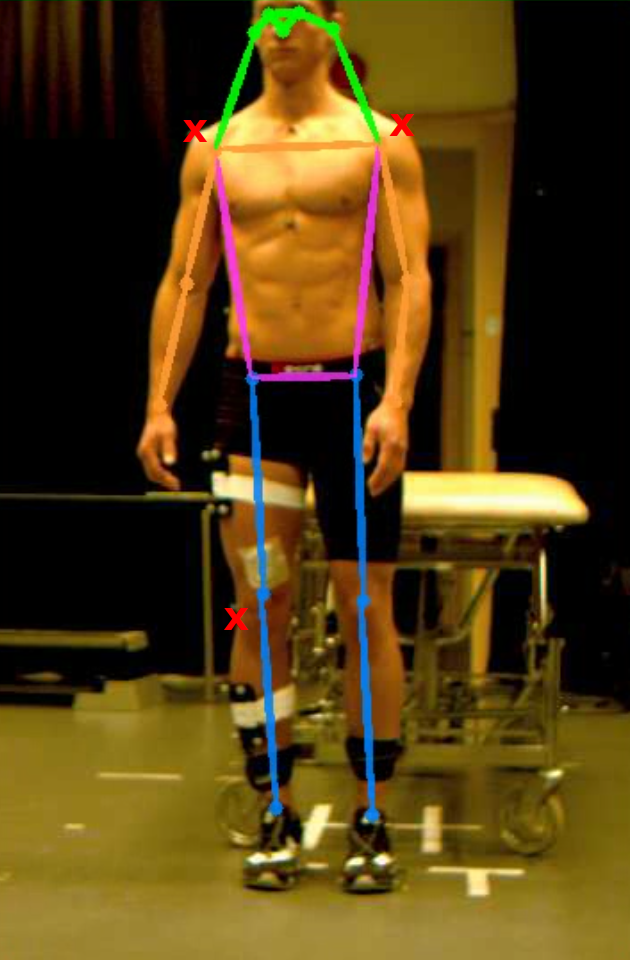
\includegraphics[height=0.8\textwidth]{figs/joint-36.png}
  \caption{Body joints detected by model trained on the COCO data set. Red crosses indicate where measured joints that deviate from the estimated ones are situated.}
  \label{fig:COCO-joints}
\end{figure}

\begin{figure}
  \centering
  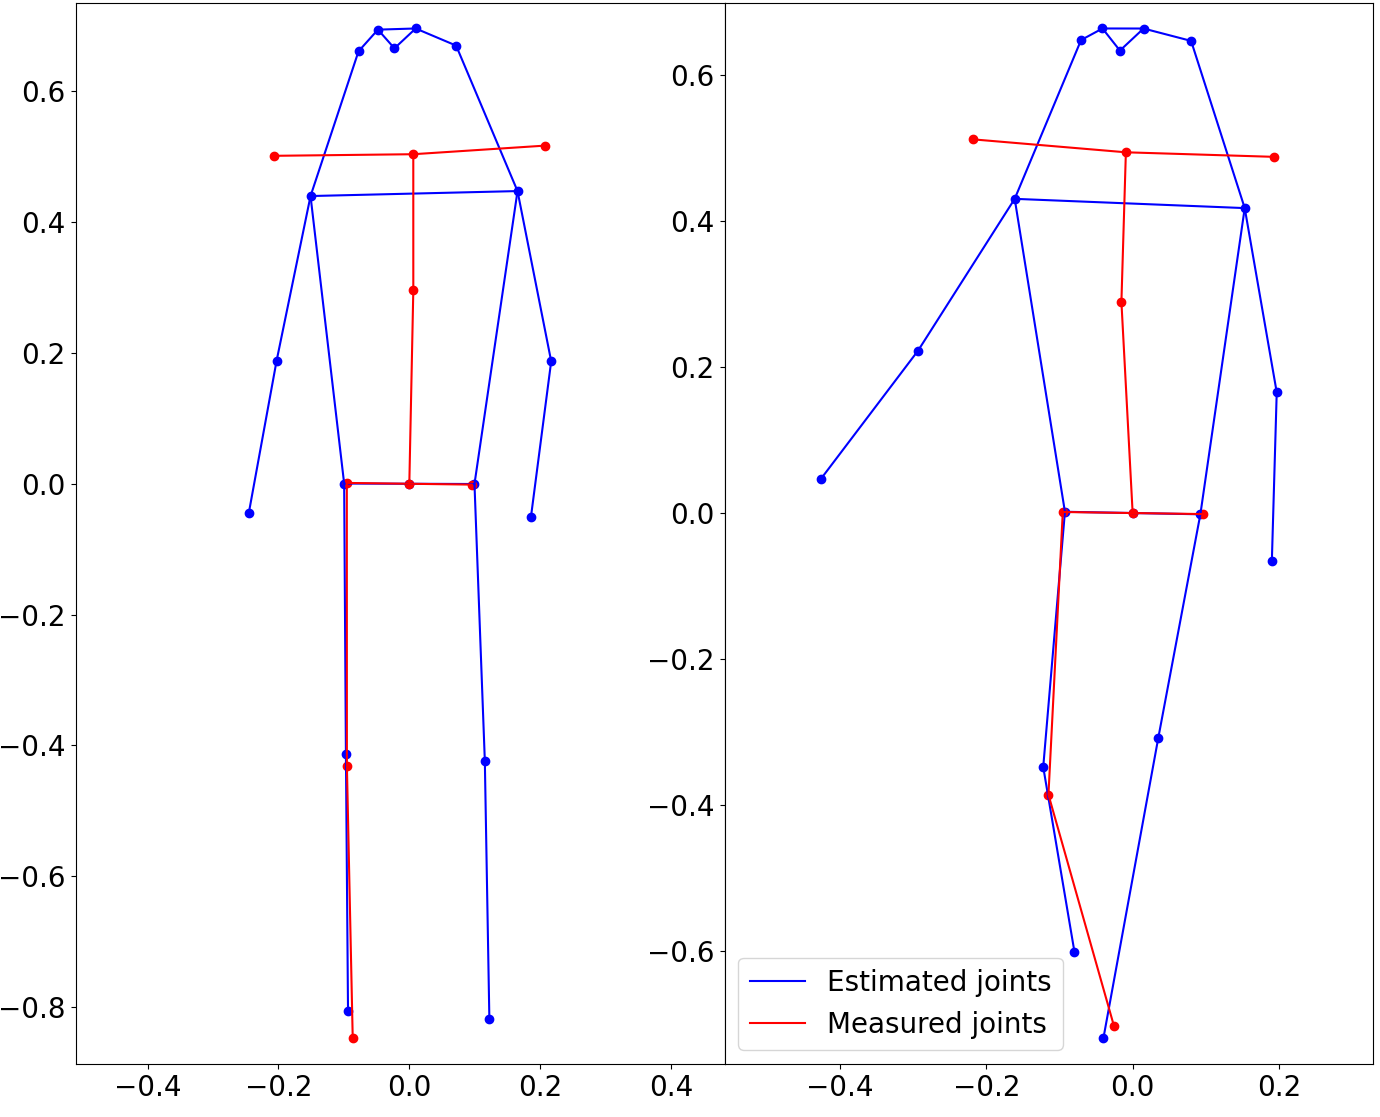
\includegraphics[height=0.8\textwidth]{figs/Figure_2.png}
  \caption{Estimated body joints together with measured joints for two frames in the video.}
  \label{fig:joints-comparison}
\end{figure}

\begin{figure}
    \centering
    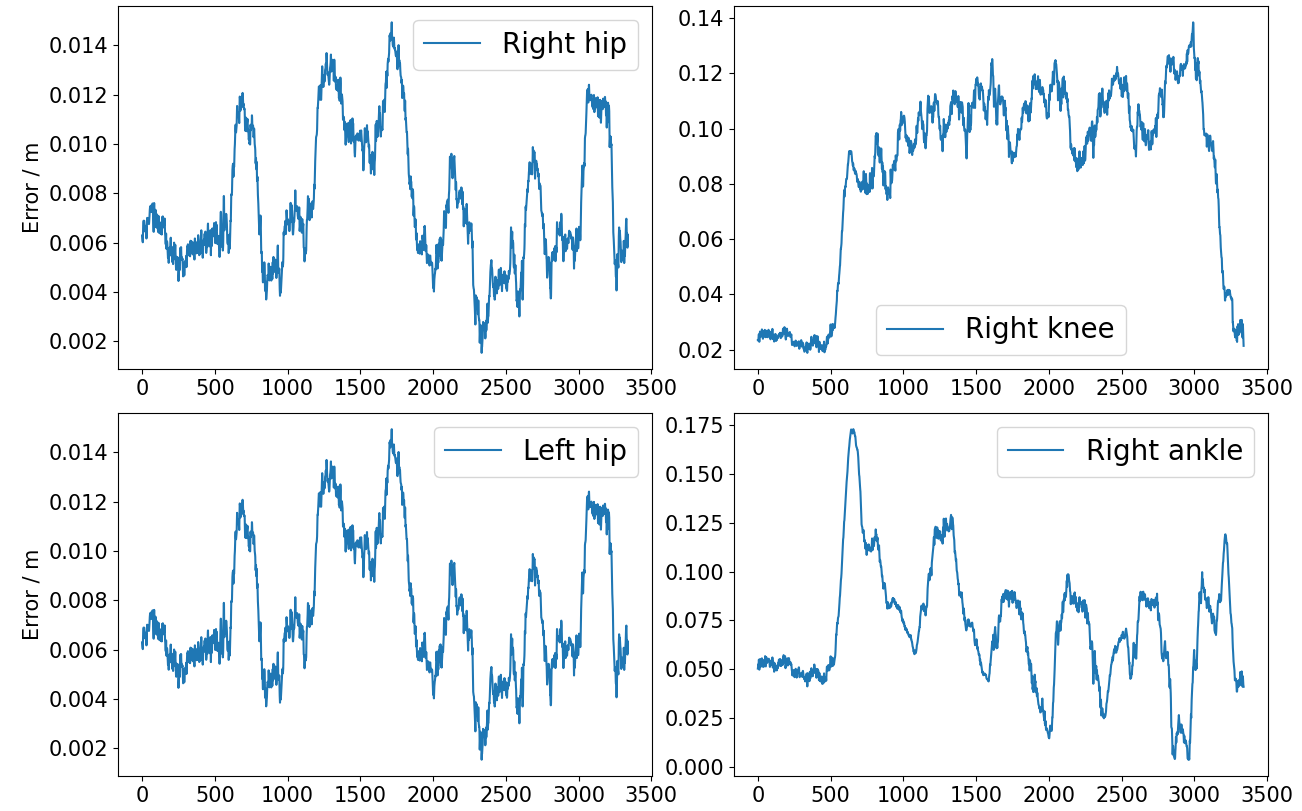
\includegraphics[width=0.9\textwidth]{figs/errrors-2d}
    \caption{Euclidean distance between the measured and estimated joint positions.}
    \label{fig:errors-2d}
\end{figure}

\begin{figure}
  \centering
  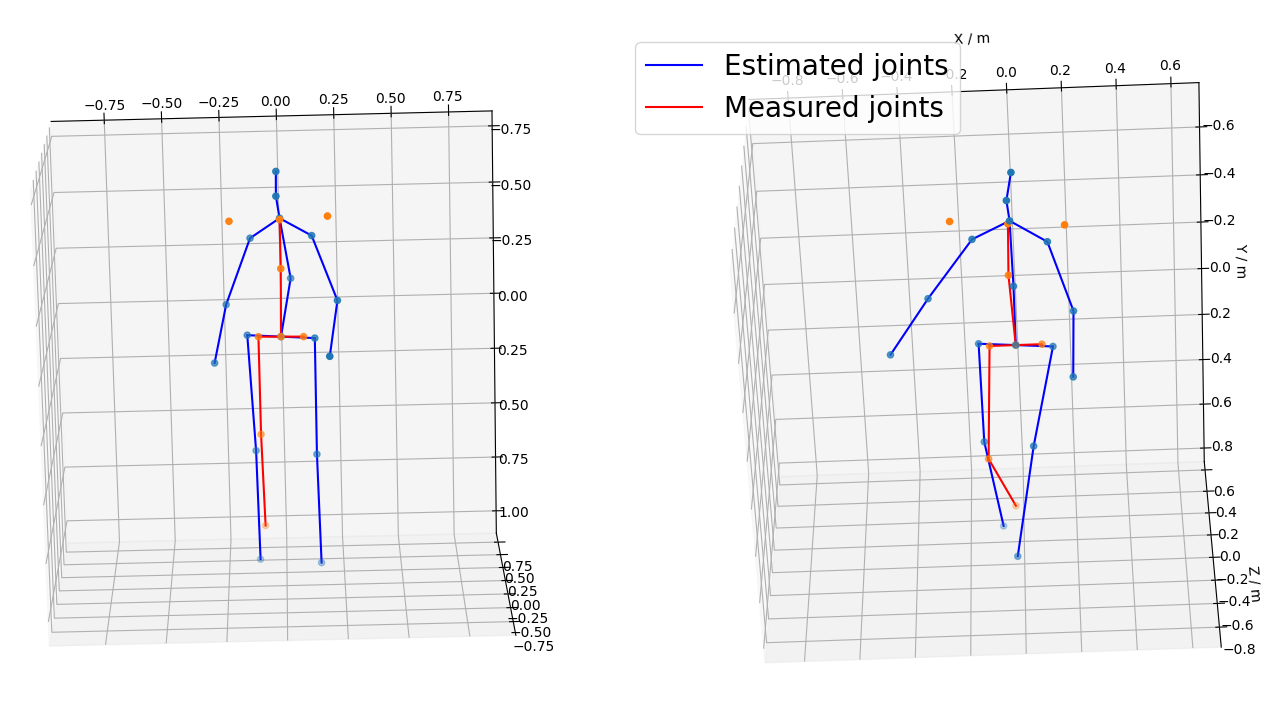
\includegraphics[width=\textwidth]{figs/joints-3d}
  \caption{Estimated 3D body joints together with measured joints for the same two frames as in Figure \ref{fig:joints-comparison}.}
  \label{fig:joints-comp3d}
\end{figure}

\begin{figure}
    \centering
    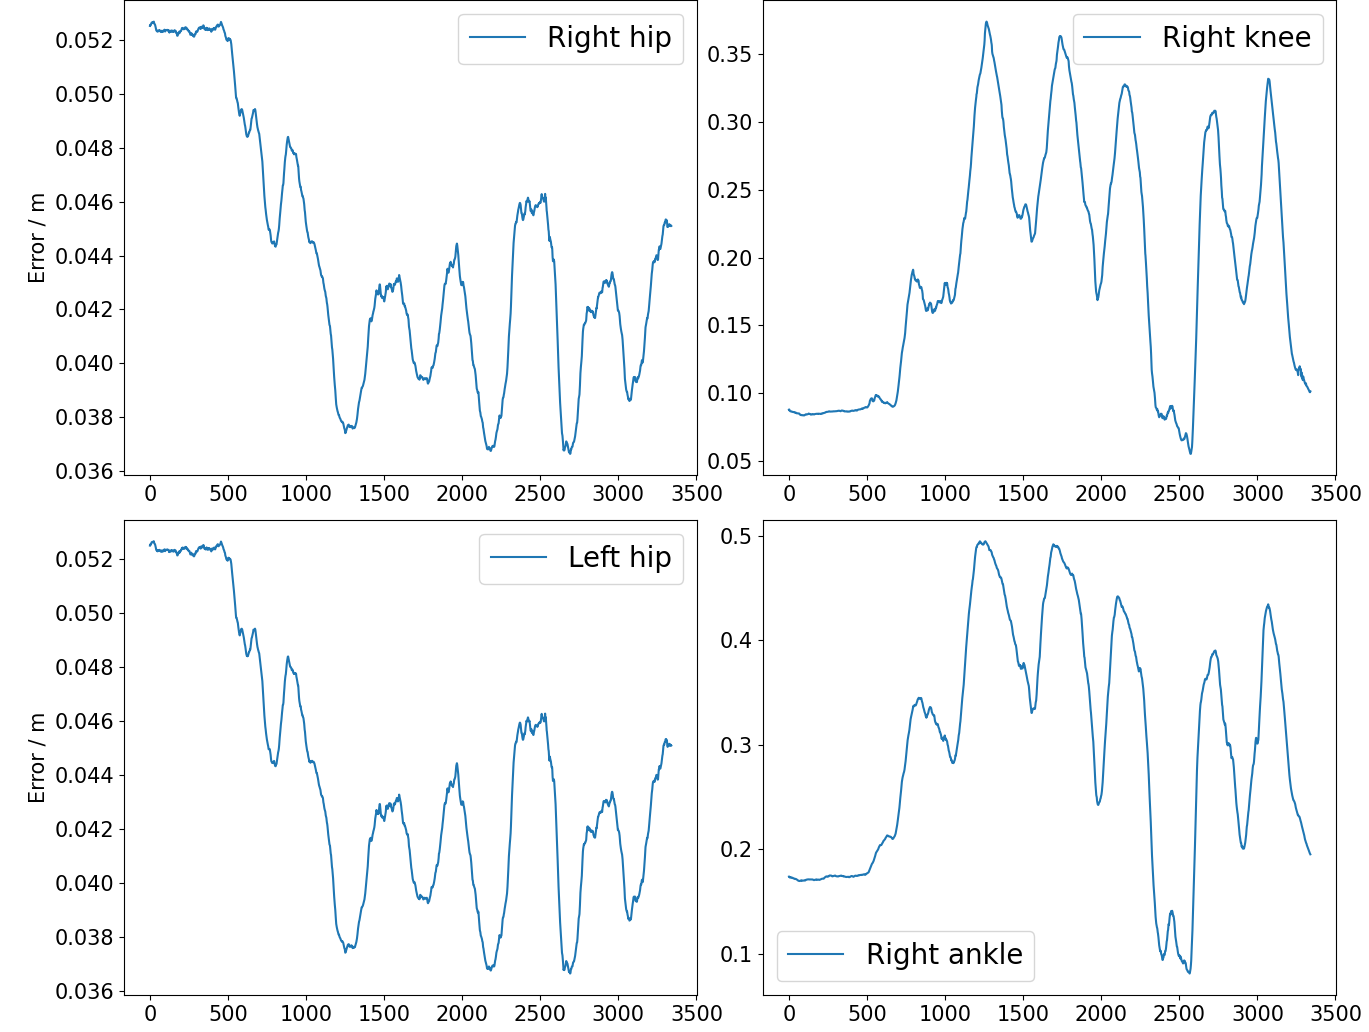
\includegraphics[width=0.9\textwidth]{figs/errors-3d}
    \caption{Euclidean distance between the measured and estimated 3D joint positions.}
    \label{fig:errors-3d}
\end{figure}

% \begin{figure}
%   \centering
%   \begin{subfigure}[t]{0.33\textwidth}
%     \includegraphics[width=\textwidth]{figs/joints-COCO}
%     \caption{Body joints detected by model trained on the COCO data set.}
%     \label{fig:COCO-joints}
%   \end{subfigure}
%   \begin{subfigure}[t]{0.66\textwidth}
%     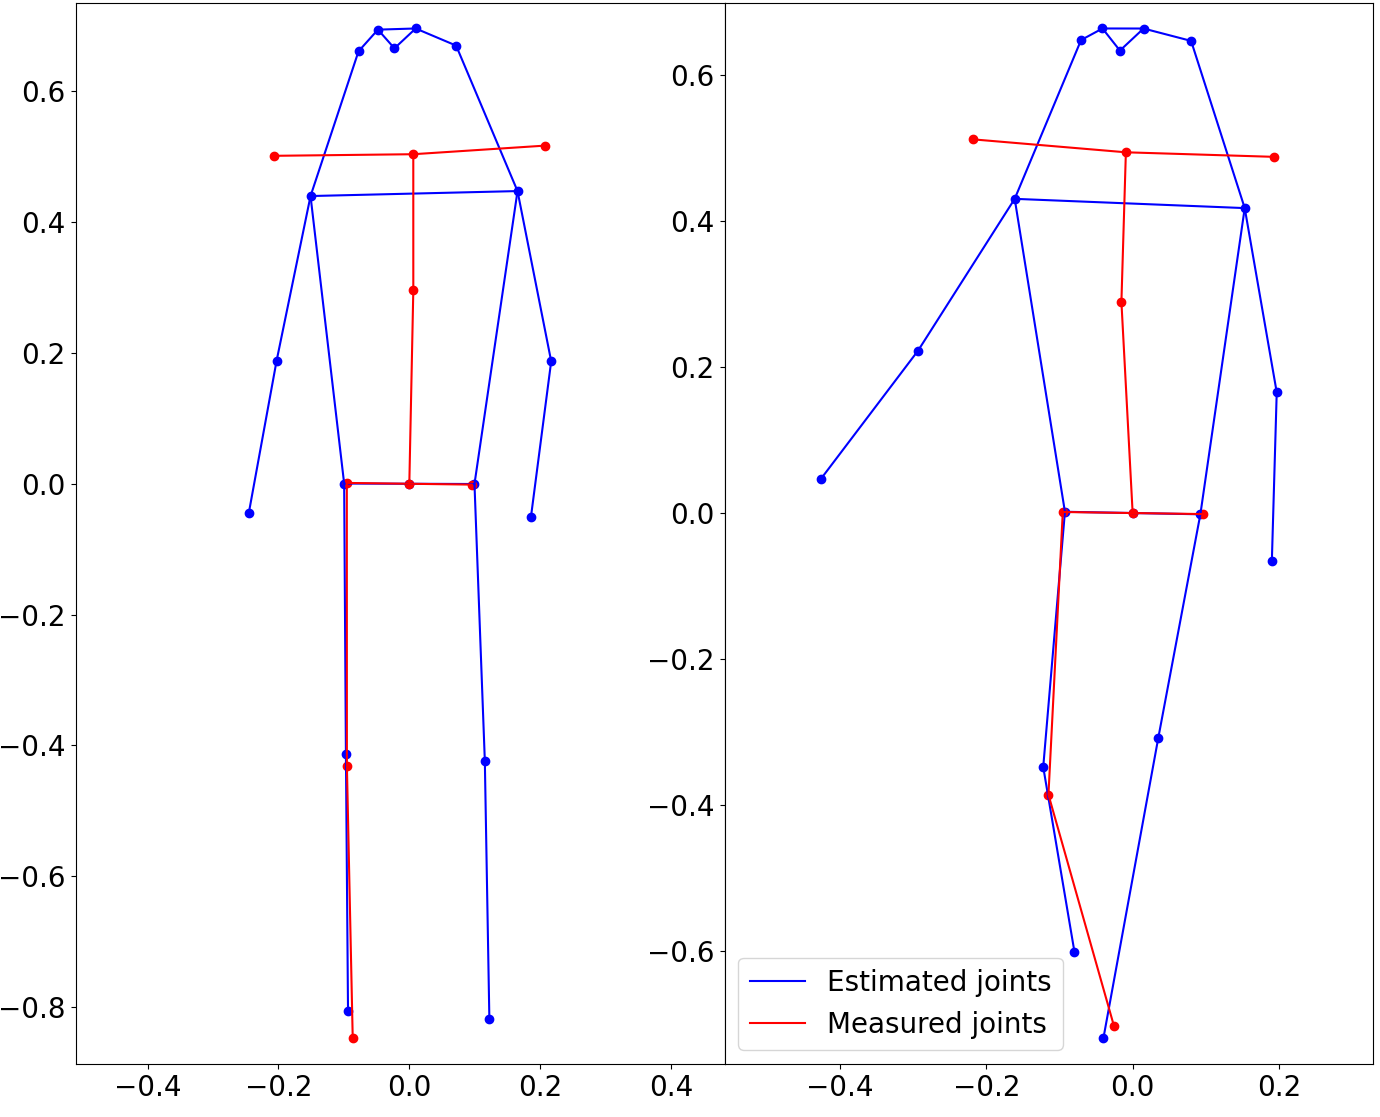
\includegraphics[width=\textwidth]{figs/Figure_2}
%     \caption{Estimated body joints together with measured joints for two frames in the video.}
%     \label{fig:COCO-joints}
%   \end{subfigure}
% \end{figure}


\newpage
\bibliography{bibtex/bib}
\bibliographystyle{plain}

\end{document}
